% ###################################
%      Chromatic Amplitude Detuning
\section{\review{Chromatic Amplitude Detuning}}

The Chromatic Amplitude Detuning is the tune shift dependant on both the actions and the momentum
offset, whose decapole contributed terms are described via a Taylor expansion in
\cref{eq:decapoles:chromatic_ampdet:decapole_contribution}. More information and derivations can
be found in \cref{subsection:detuning_effects:chromatic_amplitude_detuning} and
\cref{appendix:chromatic_amplitude_detuning}.

\begin{equation}
  \begin{aligned}
    \Delta Q(J_x, J_y, \delta) = 
    & \frac{\partial^2Q}{\partial J_x \partial \delta}    \cdot J_x\delta 
    + \frac{\partial^2 Q}{\partial J_y \partial \delta}   \cdot J_y\delta 
    + \frac{1}{3!} \frac{\partial^3 Q}{\partial \delta^3} \cdot \delta^3.
    \end{aligned}
    \label{eq:decapoles:chromatic_ampdet:decapole_contribution}
\end{equation}


The last term is more commonly referred to as the third order chromaticity, $Q'''$.  Each of these
terms depend on the $\beta$-functions, the horizontal dispersion $D_x$ and the normalized decapole
field gradient $K_5$ for a single source of length $L$,

\begin{equation}\begin{aligned}
  \frac{\partial^2 Q_x}{\partial J_x \partial \delta} =& \frac{1}{16 \pi} K_5L \beta_x^2 D_x,         &\quad
  \frac{\partial^2 Q_y}{\partial J_y \partial \delta} =& \frac{1}{16 \pi} K_5L \beta_y^2 D_x,
\\
  \frac{\partial^2 Q_x}{\partial J_y \partial \delta} =& -\frac{1}{8\pi} K_5L \beta_x \beta_y D_x,    &\quad
  \frac{\partial^2 Q_y}{\partial J_x \partial \delta} =& -\frac{1}{8\pi} K_5L \beta_x \beta_y D_x,
\\
  \frac{\partial^3 Q_x}{\partial \delta^3}            =& \frac{1}{4\pi} K_5L \beta_x D_x^3,           &\quad
  \frac{\partial^3 Q_y}{\partial \delta^3}            =& -\frac{1}{4\pi} K_5L \beta_y D_x^3.
\end{aligned}\end{equation}

Notably, while the $K_5$ dependence is identical to that of $Q'''$, the $\beta$ and $D_x$
dependencies differ significantly. In the presence of a systematic error in the magnetic model, one
would expect similar ratios for this observable as those observed for $Q'''$.
The action dependant terms can be measured by exciting the beam with an AC-dipole with increasing
strengths at different momentum-offsets. The AC-Dipole introduces effects that are corrected in the
analysis~\cite{dilly_corrections_2022}.

Such a measurement was taken with octupole and decapole correctors turned off to measure the bare
machine. The momentum-offsets measured at were $-0.001$ and $0.001$, respectively roughly equal to
a trim of $+140$Hz and $-140$Hz of the RF. Some data could not be collected due to machine
availability issues, restricting the measurement to low amplitude kicks.
Nevertheless, the terms $\frac{\partial^2 Q_x}{\partial J_y \partial \delta}$ and $\frac{\partial^2
Q_y}{\partial J_y \partial \delta}$ for beam 2 were successfully measured for the first time in the
LHC. 

\Cref{figure:decapoles:chromatic_amplitude_detuning:b2qxy}
and~\cref{figure:decapoles:chromatic_amplitude_detuning:b2qyy} show a fit of those terms to measured
$Q_{x,y}$ vs $J_{y}$ at two different momentum offsets. Expected shifts from MADX-PTC simulations,
that include field errors ranging from sextupoles to decahexapoles ($b_3$ to $b_8$ and $a_4$ to
$a_8$) are shown as a comparison.

% Studies and plots in 
% jupyter/chromatic_amplitude_detuning/simulations/2022-10-19_vs_PTC/Analytical_Chromatic_Detuning.ipynb

\begin{figure}[H]
  \centering
  \begin{subfigure}{0.8\textwidth}
      \centering
      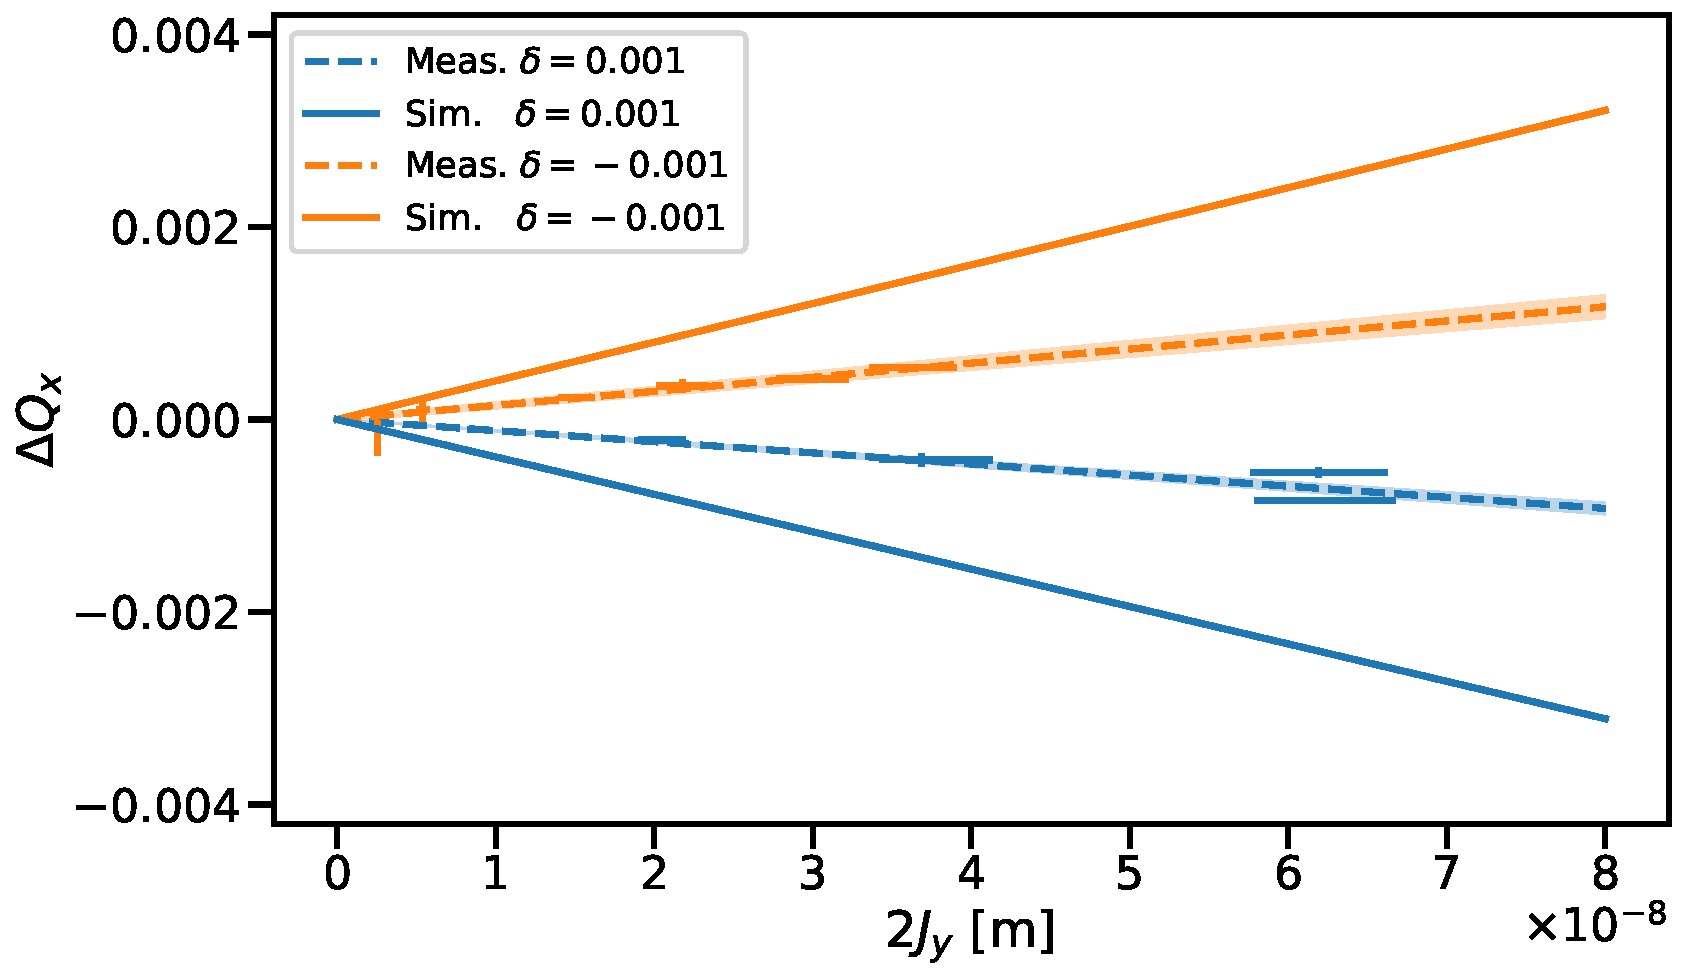
\includegraphics[width=\textwidth]{images/chromatic_amplitude_detuning/B2_Qxy_decay0.00.pdf}
      \caption{Horizontal tune shift depending on the vertical action: 
      $\frac{\partial^2 Q_x}{\partial J_y \partial \delta}$.}
      \label{figure:decapoles:chromatic_amplitude_detuning:b2qxy}
  \end{subfigure}
  %
  \\[1em]
  %
  \begin{subfigure}{0.8\textwidth}
      \centering
      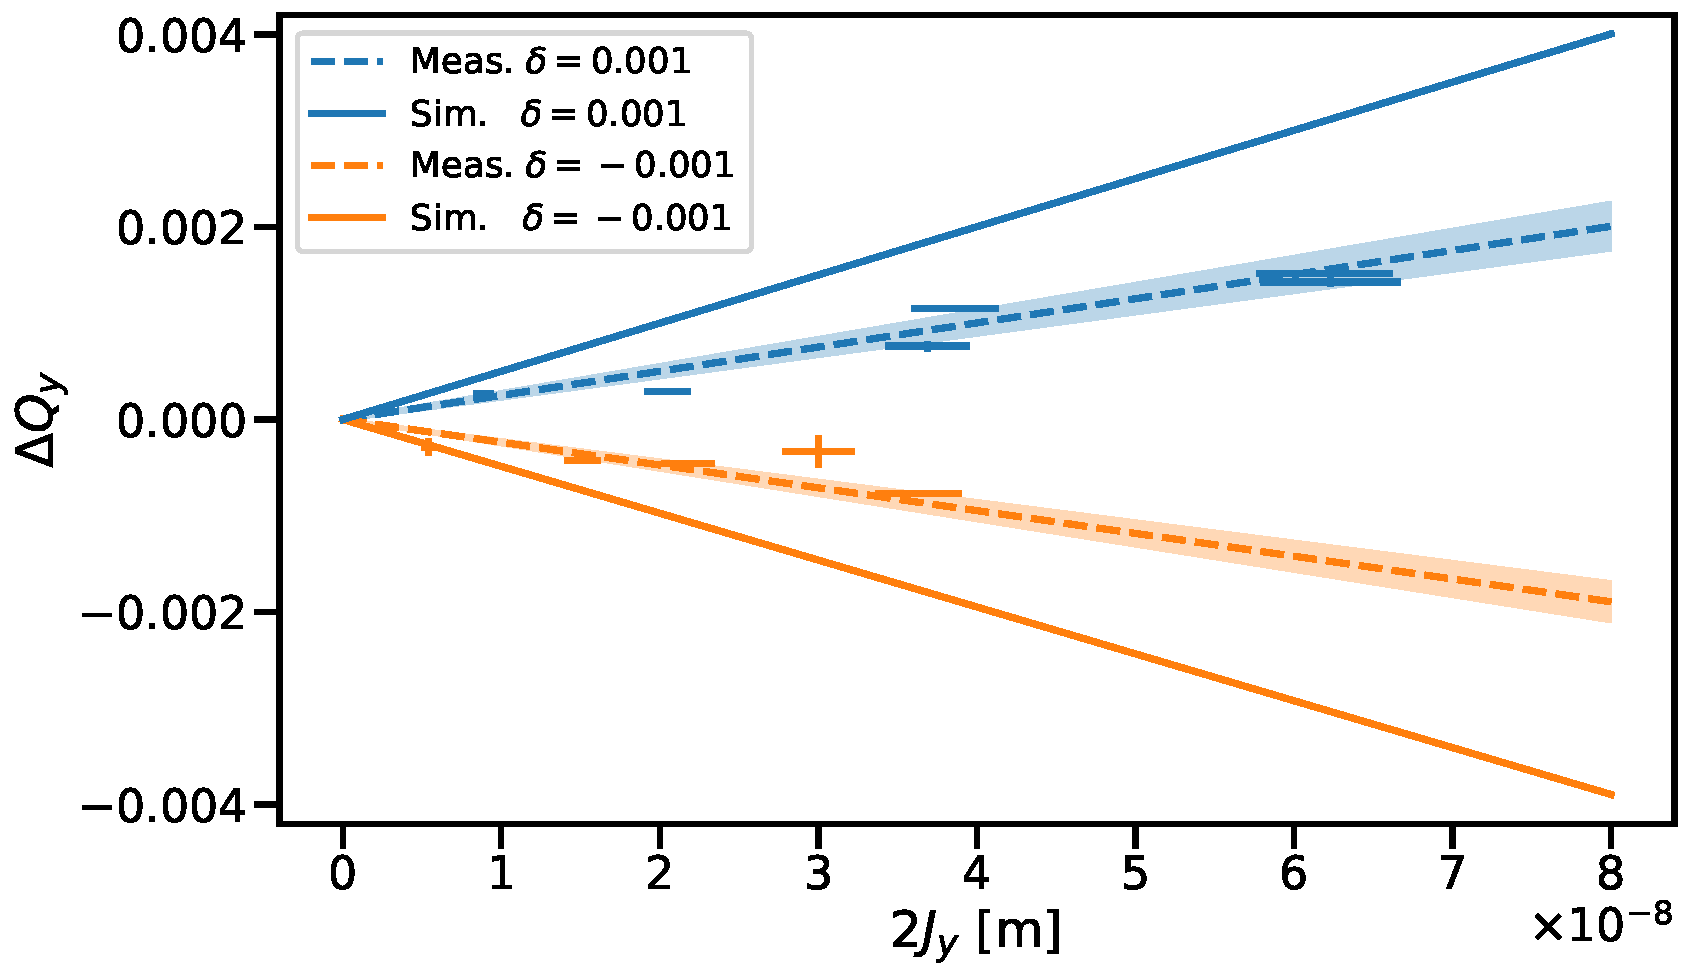
\includegraphics[width=\textwidth]{images/chromatic_amplitude_detuning/B2_Qyy_decay0.00.pdf}
      \caption{Vertical tune shift depending on the vertical action: 
      $\frac{\partial^2 Q_y}{\partial J_y \partial \delta}$.}
      \label{figure:decapoles:chromatic_amplitude_detuning:b2qyy}
  \end{subfigure}
  \caption{Measured and simulated tune shift due to a change of action via an AC-Dipole at two
  different momentum offsets. Each fit corresponds to a chromatic amplitude detuning term evaluated
  at a certain $\delta$.}
  \label{figure:decapoles:chromatic_amplitude_detuning:two_terms}
\end{figure}

\begin{table}[H]
  \centering
  \begin{tabular}{lrr}
  \toprule
   Type  & $\frac{\partial^2 Q_x}{\partial J_y \partial \delta}[10^{4}\mathrm{m}^{-1}]$ & $\frac{\partial^2 Q_y}{\partial J_y \partial \delta}[10^{4}\mathrm{m}^{-1}]$ \\
  \midrule
  $\delta = +0.001$ & & \\
  \hspace{2mm}Meas.  &   -1.16 ± 0.08 &   1.26 ± 0.15 \\
  \hspace{2mm}Sim.   &   -3.82 ± 0.01 &   2.47 ± 0.01 \\
  \hspace{2mm}Ratio  &    0.30 ± 0.02 &   0.51 ± 0.06 \\
  $\delta = -0.001$ & & \\
  \hspace{2mm}Meas.  &  1.47 ± 0.12  &  -1.18 ± 0.13 \\
  \hspace{2mm}Sim.   &  3.92 ± 0.01  &  -2.41 ± 0.01 \\
  \hspace{2mm}Ratio  &  0.38 ± 0.03  &   0.49 ± 0.05 \\
  \bottomrule
  \end{tabular}
  \caption{Comparison of the measured and simulated terms $\frac{\partial^2 Q_x}{\partial J_y
   \delta}$ and $\frac{\partial^2 Q_y}{\partial J_y \partial \delta}$ via PTC, at two
  discrete momentum offsets. Simulations include errors from normal sextupole to decahexapole and
  from skew octupole to decahexapole.}
  \label{table:decapoles:chromatic_ampdet}
\end{table}


A similar ratio between simulation and measurement is observed accross the different terms. The
values and ratios of measurement to model can be found in \cref{table:decapoles:chromatic_ampdet}.
The observed ratios for the chromatic amplitude detuning are quite similar, while not exact,
to those of the bare chromaticity.
This similarity of the ratios between the chromatic amplitude detuning and $Q'''$ discrepancies
suggests an issue with the decapolar error model of the main dipoles, with measurements showing
values about half of those predicted by the magnetic model.
